\documentclass[12pt,a4paper]{article}
\usepackage{graphicx}
\usepackage{float}
\usepackage[utf8]{vietnam}
\usepackage{geometry}
\usepackage{hyperref}
\usepackage{enumitem}
\usepackage{tabularx}
\geometry{
    a4paper,
    margin=1in
}

\setlist[itemize]{leftmargin=1.5cm}
\setlist[enumerate]{leftmargin=1.5cm}

\title{\textbf{PHÂN TÍCH NGƯỜI DÙNG VÀ USECASE}\\
\Large ĐỒ ÁN 1 (15/10/2026)}
\author{\textbf{Đề tài:} Xây dựng website thương mại điện tử\\
bán máy tính và linh kiện máy tính}

\date{}

\begin{document}

\maketitle
\section{PHẠM VI HỆ THỐNG}

Hệ thống được xây dựng nhằm hỗ trợ hoạt động kinh doanh máy tính và linh kiện máy tính thông qua website thương mại điện tử. Người dùng có thể xem, tìm kiếm và lựa chọn sản phẩm, quản lý giỏ hàng, đặt hàng và thanh toán. Hệ thống cũng hỗ trợ quản lý đơn hàng, sản phẩm, danh mục, người dùng, kho và thống kê.

Phạm vi của hệ thống tập trung vào các chức năng cốt lõi của website bán lẻ, bao gồm xác thực tài khoản, tra cứu và phân loại sản phẩm, quản lý giá khuyến mãi, voucher, đơn hàng, địa chỉ giao hàng, kho và thống kê. AI, chatbot, đa nhà bán hàng, tích điểm, đánh giá sản phẩm và tích hợp vận chuyển phức tạp không thuộc phạm vi hiện tại.

\section{PHÂN TÍCH NGƯỜI DÙNG (ACTOR)}

\begin{itemize}

 \item \textbf{Khách vãng lai:} Là người truy cập website nhưng chưa được xác thực đăng nhập vào hệ thống. Khách vãng lai có thể đã có hoặc chưa có tài khoản. Actor này chỉ có quyền đăng ký, đăng nhập, xem, tìm kiếm và lọc sản phẩm. Nếu muốn thực hiện thao tác với giỏ hàng hoặc mua hàng, hệ thống sẽ yêu cầu Khách vãng lai phải đăng nhập để chuyển thành Khách hàng.

 \item \textbf{Khách hàng:} Là người đã có tài khoản và đăng nhập vào hệ thống. Khách hàng có thể xem sản phẩm, quản lý giỏ hàng, đặt hàng, thanh toán, theo dõi và hủy đơn hàng theo điều kiện cho phép, đồng thời quản lý thông tin tài khoản.

 \item \textbf{Nhân viên:} Là người hỗ trợ hoạt động bán hàng và xử lý đơn hàng. Nhân viên có thể xem và xử lý đơn hàng trong phạm vi quyền được cấp, đồng thời kiểm tra số lượng tồn kho của sản phẩm. Nhân viên không có quyền trực tiếp điều chỉnh tồn kho.

 \item \textbf{Quản trị viên:} Là người có quyền quản lý và vận hành hệ thống. Quản trị viên có thể quản lý đơn hàng, sản phẩm, danh mục, người dùng, kho và xem các số liệu thống kê.

 \item \textbf{Cổng thanh toán:} Là hệ thống bên ngoài được sử dụng để xử lý các giao dịch thanh toán trực tuyến và trả kết quả giao dịch về cho hệ thống.

 \item \textbf{Google Identity:} Là nhà cung cấp danh tính bên ngoài, xác thực người dùng và trả thông tin định danh đã được xác minh cho hệ thống khi người dùng chọn đăng nhập bằng Google.

\end{itemize}

\section{DANH SÁCH USE CASE CHÍNH}

\begin{itemize}
    \item \textbf{UC01: Đăng ký}
    \item \textbf{UC02: Đăng nhập}
    \item \textbf{UC03: Xem, tìm kiếm và lọc sản phẩm}
    \item \textbf{UC04: Quản lý giỏ hàng}
    \item \textbf{UC05: Đặt hàng}
    \item \textbf{UC06: Thanh toán}
    \item \textbf{UC07: Theo dõi và hủy đơn hàng}
    \item \textbf{UC08: Quản lý tài khoản}
    \item \textbf{UC09: Quản lý đơn hàng}
    \item \textbf{UC10: Kiểm tra tồn kho}
    \item \textbf{UC11: Quản lý sản phẩm}
    \item \textbf{UC12: Quản lý danh mục}
    \item \textbf{UC13: Quản lý người dùng}
    \item \textbf{UC14: Quản lý kho}
    \item \textbf{UC15: Xem thống kê}
    \item \textbf{UC16: Quản lý chương trình giảm giá}
    \item \textbf{UC17: Quản lý voucher}
    \item \textbf{UC18: Áp dụng voucher khi đặt hàng}
\end{itemize}

\section{QUY TRÌNH NGHIỆP VỤ CHUNG}

\subsection{Quy trình xử lý đơn hàng}

Quy trình xử lý đơn hàng trong hệ thống được xác định như sau:

\begin{center}
Chờ xác nhận $\rightarrow$ Đang chuẩn bị hàng $\rightarrow$ Đang giao hàng $\rightarrow$ Hoàn thành / Giao hàng thất bại
\end{center}

Ngoài luồng xử lý chính, đơn hàng có thể chuyển từ trạng thái \textbf{Chờ xác nhận} sang \textbf{Đã hủy} khi khách hàng thực hiện hủy đơn theo điều kiện cho phép, hoặc hệ thống tự động hủy do thanh toán không thành công hoặc quá thời gian thanh toán quy định.
\subsection{Quy tắc chuyển trạng thái đơn hàng}

\begin{itemize}
\item \textbf{Chờ xác nhận $\rightarrow$ Đang chuẩn bị hàng:} Nhân viên hoặc Quản trị viên xác nhận đơn hàng sau khi kiểm tra thông tin hợp lệ.

\item \textbf{Chờ xác nhận $\rightarrow$ Đã hủy:} Khách hàng được phép hủy đơn khi đơn hàng chưa được xác nhận; hệ thống tự động hủy đơn khi giao dịch thanh toán không thành công hoặc quá thời gian thanh toán quy định.

\item \textbf{Đang chuẩn bị hàng $\rightarrow$ Đang giao hàng:} Đơn hàng đã được chuẩn bị và chuyển sang quá trình giao hàng.

\item \textbf{Đang giao hàng $\rightarrow$ Hoàn thành:} Đơn hàng hoàn tất quá trình giao hàng thành công.

\item \textbf{Đang giao hàng $\rightarrow$ Giao hàng thất bại:} Giao hàng không thành công, chẳng hạn khách hàng từ chối nhận hàng hoặc shipper không thể liên lạc; đơn hàng được xử lý hoàn về kho.

\item Không cho phép chuyển trạng thái tùy ý; trạng thái mới phải phù hợp với quy trình xử lý đơn hàng.

\item Đơn hàng đã ở trạng thái \textbf{Đã hủy}, \textbf{Giao hàng thất bại} hoặc \textbf{Hoàn thành} không được chuyển sang trạng thái xử lý khác.
\end{itemize}

\subsection{Quy tắc hủy đơn hàng}
\begin{itemize}
    \item Khách hàng chỉ được phép hủy đơn khi đơn hàng đang ở trạng thái \textbf{Chờ xác nhận}.
    \item Khách hàng không được phép tự hủy đơn khi đơn hàng đang ở trạng thái \textbf{Đang chuẩn bị hàng}, \textbf{Đang giao hàng} hoặc \textbf{Hoàn thành}.
    \item Đơn hàng đã ở trạng thái \textbf{Đã hủy} không thể thực hiện thao tác hủy lại.
\end{itemize}

\subsection{Quy tắc quản lý tồn kho}

\begin{itemize}
\item Khi khách hàng đặt hàng thành công (tạo đơn hàng), hệ thống sẽ ngay lập tức \textbf{tạm trừ (giữ chỗ)} số lượng tồn kho của các sản phẩm tương ứng.
\item Không cho phép tạo đơn hàng nếu số lượng tồn kho hiện tại không đủ đáp ứng số lượng trong giỏ hàng.
\item Nếu đơn hàng chuyển sang trạng thái \textbf{Đã hủy} (do khách hàng hủy hoặc hệ thống tự động hủy do quá hạn thanh toán), hệ thống sẽ tự động \textbf{cộng trả lại} số lượng tồn kho đã tạm trừ.
\item Nếu đơn hàng chuyển sang trạng thái \textbf{Giao hàng thất bại}, hệ thống sẽ \textbf{cộng trả lại} số lượng tồn kho sau khi xác nhận hàng hoàn về kho.
\item Việc kiểm tra và tạm trừ tồn kho ngay tại thời điểm khách hàng đặt hàng giúp tránh tình trạng nhiều khách hàng cùng đặt một sản phẩm trong khi số lượng tồn kho có hạn.
\item Hệ thống không cho phép số lượng tồn kho nhỏ hơn 0.
\end{itemize}


\subsection{Quy tắc thanh toán}

Hệ thống hỗ trợ hai phương thức thanh toán cơ bản:

\begin{itemize}
    \item \textbf{Thanh toán khi nhận hàng (COD):} Khi đơn hàng được tạo, trạng thái thanh toán được ghi nhận là \textbf{Chưa thanh toán}. Khách hàng thực hiện thanh toán khi nhận hàng. Khi giao dịch COD được hoàn tất thành công, trạng thái thanh toán của đơn hàng được cập nhật thành \textbf{Đã thanh toán}.

    \item \textbf{Thanh toán trực tuyến:} Hệ thống gửi yêu cầu giao dịch đến Cổng thanh toán. Chỉ khi nhận được kết quả giao dịch hợp lệ và thành công, hệ thống mới cập nhật trạng thái thanh toán thành \textbf{Đã thanh toán}.
\end{itemize}

Trạng thái thanh toán gồm:

\begin{itemize}
    \item \textbf{Chưa thanh toán:} Đơn hàng chưa ghi nhận thanh toán thành công.
    \item \textbf{Đã thanh toán:} Đơn hàng đã ghi nhận thanh toán thành công.
\end{itemize}

\subsection{Quy tắc xử lý thanh toán trực tuyến thất bại}

\begin{itemize}
    \item Nếu giao dịch trực tuyến thất bại hoặc bị khách hàng hủy, hệ thống giữ trạng thái thanh toán là \textbf{Chưa thanh toán} và thông báo kết quả cho khách hàng.

    \item Đối với đơn hàng vẫn còn hiệu lực và đang ở trạng thái chưa thanh toán, khách hàng được phép thực hiện lại thao tác thanh toán trực tuyến.

    \item Hệ thống không tự động chuyển trạng thái thanh toán thành \textbf{Đã thanh toán} nếu chưa nhận được kết quả giao dịch thành công hợp lệ từ Cổng thanh toán.

    \item Đơn hàng đã ở trạng thái \textbf{Đã thanh toán} không được thực hiện thanh toán lại.

    \item Đơn hàng đã ở trạng thái \textbf{Đã hủy} không được thực hiện thanh toán.

    \item Việc chuyển đổi từ thanh toán trực tuyến sang COD chỉ được thực hiện nếu hệ thống có hỗ trợ chức năng thay đổi phương thức thanh toán.
\end{itemize}

\section{ĐẶC TẢ CHI TIẾT CÁC USE CASE}

% ==================================================

\subsection{UC01. Đăng ký}

\begin{itemize}
    \item \textbf{Actor:} Khách vãng lai.
    \item \textbf{Mục tiêu:} Cho phép khách vãng lai tạo tài khoản mới để sử dụng các chức năng dành cho khách hàng.
    \item \textbf{Mô tả:} Use Case này cho phép người dùng chưa đăng nhập đăng ký tài khoản mới bằng cách cung cấp các thông tin cần thiết. Hệ thống kiểm tra tính đầy đủ, hợp lệ và tính duy nhất của thông tin trước khi tạo tài khoản.
    \item \textbf{Điều kiện trước:} Người dùng chưa đăng nhập vào hệ thống.
    \item \textbf{Luồng chính:}
    \begin{enumerate}
        \item Người dùng chọn chức năng Đăng ký.
        \item Hệ thống hiển thị biểu mẫu đăng ký.
        \item Người dùng nhập các thông tin cần thiết.
        \item Người dùng gửi thông tin đăng ký.
        \item Hệ thống kiểm tra tính đầy đủ và hợp lệ của thông tin.
        \item Hệ thống kiểm tra tài khoản đã tồn tại hay chưa.
        \item Hệ thống tạo tài khoản mới.
        \item Hệ thống thông báo đăng ký thành công.
    \end{enumerate}
    \item \textbf{Luồng thay thế / Ngoại lệ:}
    \begin{itemize}
        \item Nếu thông tin chưa đầy đủ, hệ thống thông báo và yêu cầu người dùng bổ sung thông tin.
        \item Nếu thông tin không hợp lệ, hệ thống thông báo lỗi và yêu cầu người dùng kiểm tra, nhập lại thông tin.
        \item Nếu tài khoản đã tồn tại, hệ thống thông báo tài khoản đã tồn tại và yêu cầu người dùng sử dụng thông tin khác.
    \end{itemize}
    \item \textbf{Điều kiện sau:} Tài khoản mới được tạo thành công.
    \item \textbf{Quy tắc nghiệp vụ:}
    \begin{itemize}
        \item Thông tin đăng ký phải đầy đủ và hợp lệ.
        \item Thông tin định danh tài khoản không được trùng với tài khoản đã tồn tại.
    \end{itemize}
\end{itemize}

% ==================================================

\subsection{UC02. Đăng nhập}

\begin{itemize}
    \item \textbf{Actor:} Khách vãng lai, Google Identity.
    \item \textbf{Mục tiêu:} Cho phép người dùng xác thực tài khoản và đăng nhập vào hệ thống.
    \item \textbf{Mô tả:} Use Case này cho phép người dùng cung cấp thông tin đăng nhập. Hệ thống kiểm tra thông tin xác thực và trạng thái tài khoản trước khi thiết lập trạng thái đăng nhập.
    \item \textbf{Điều kiện trước:} Người dùng chưa đăng nhập vào hệ thống.
    \item \textbf{Luồng chính:}
    \begin{enumerate}
        \item Người dùng chọn chức năng Đăng nhập.
        \item Hệ thống hiển thị biểu mẫu đăng nhập bằng tài khoản hệ thống và lựa chọn đăng nhập bằng Google.
        \item Người dùng chọn một phương thức đăng nhập. Với tài khoản hệ thống, người dùng nhập tên đăng nhập/email và mật khẩu rồi gửi biểu mẫu.
        \item Hệ thống kiểm tra thông tin đăng nhập hoặc chuyển người dùng đến Google Identity để xác thực.
        \item Nếu xác thực qua Google thành công, Google Identity trả thông tin định danh đã xác minh về hệ thống; hệ thống tìm tài khoản Google đã liên kết hoặc tạo tài khoản Khách hàng mới theo quy tắc nghiệp vụ.
        \item Hệ thống kiểm tra trạng thái tài khoản.
        \item Hệ thống thiết lập trạng thái đăng nhập.
        \item Hệ thống thông báo đăng nhập thành công và điều hướng người dùng theo vai trò.
    \end{enumerate}
    \item \textbf{Luồng thay thế / Ngoại lệ:}
    \begin{itemize}
        \item Nếu thông tin đăng nhập chưa đầy đủ, hệ thống thông báo dữ liệu chưa đầy đủ và yêu cầu người dùng nhập lại.
        \item Nếu tài khoản không tồn tại, hệ thống thông báo tài khoản không tồn tại và cho phép người dùng chuyển sang UC01 -- Đăng ký.
        \item Nếu mật khẩu không chính xác, hệ thống thông báo mật khẩu không đúng và yêu cầu người dùng nhập lại.
        \item Nếu người dùng hủy xác thực Google, Google Identity trả lỗi hoặc thông tin xác thực không hợp lệ, hệ thống từ chối đăng nhập và thông báo phù hợp.
        \item Nếu email Google đã thuộc một tài khoản hiện có nhưng chưa được liên kết, hệ thống không tự động gộp tài khoản; người dùng phải xác thực tài khoản hiện có để liên kết.
        \item Nếu tài khoản ở trạng thái \textbf{Không còn hoạt động}, hệ thống thông báo tài khoản không tồn tại và từ chối đăng nhập.
        \item Nếu tài khoản ở trạng thái \textbf{Bị vô hiệu hóa}, hệ thống thông báo tài khoản đã bị vô hiệu hóa và từ chối đăng nhập.
        \item Nếu không thể thiết lập trạng thái đăng nhập, hệ thống thông báo xảy ra lỗi trong quá trình đăng nhập và yêu cầu người dùng thực hiện lại.
    \end{itemize}
    \item \textbf{Điều kiện sau:} Người dùng được xác thực và đăng nhập thành công; trạng thái đăng nhập được thiết lập. Khách hàng được chuyển đến trang chủ; Quản trị viên được chuyển đến trang tổng quan quản trị.
    \item \textbf{Quy tắc nghiệp vụ:}
    \begin{itemize}
        \item Chỉ tài khoản tồn tại và đang ở trạng thái \textbf{Hoạt động} mới được phép đăng nhập.
        \item Tài khoản bị vô hiệu hóa hoặc không còn hoạt động không được phép đăng nhập.
        \item Sau khi đăng nhập, hệ thống điều hướng theo vai trò: Khách hàng đến trang chủ; Quản trị viên đến khu vực quản trị. Người dùng đã đăng nhập truy cập lại trang đăng nhập cũng được điều hướng theo vai trò.
        \item Tài khoản mới tạo bằng Google mặc định có vai trò \textbf{Khách hàng}; thông tin từ Google không được dùng để cấp quyền Quản trị viên.
        \item Tài khoản Google được liên kết bằng mã định danh ổn định do Google cấp sau khi hệ thống xác minh chữ ký, đối tượng nhận, thời hạn và trạng thái email đã xác minh.
    \end{itemize}
\end{itemize}

% ==================================================

\subsection{UC03. Xem, tìm kiếm và lọc sản phẩm}

\begin{itemize}

 \item \textbf{Actor:} Khách vãng lai, Khách hàng.

 \item \textbf{Mục tiêu:} Cho phép người dùng tra cứu và xem thông tin sản phẩm phù hợp với nhu cầu.

 \item \textbf{Mô tả:} Use Case này cho phép người dùng xem danh sách sản phẩm mà không cần đăng nhập. Người dùng có thể tìm kiếm sản phẩm bằng từ khóa, lựa chọn danh mục, lọc theo khoảng giá hoặc thương hiệu. Sau khi tìm được sản phẩm phù hợp, người dùng có thể xem thông tin chi tiết như tên, hình ảnh, giá bán, mô tả, thông số kỹ thuật và tình trạng tồn kho.

 \item \textbf{Điều kiện trước:} Sản phẩm tồn tại và đang được phép hiển thị trên website.

 \item \textbf{Luồng chính:}

 \begin{enumerate}

  \item Người dùng truy cập khu vực hiển thị sản phẩm.

  \item Hệ thống hiển thị danh sách sản phẩm đang kinh doanh.

  \item Người dùng có thể chọn danh mục sản phẩm.

  \item Người dùng có thể nhập từ khóa tìm kiếm.

  \item Người dùng có thể lọc sản phẩm theo loại sản phẩm, thương hiệu, khoảng giá và các thuộc tính kỹ thuật được hệ thống hỗ trợ.

  \item Hệ thống hiển thị giá niêm yết, giá sau giảm và thông tin chương trình giảm giá đang có hiệu lực (nếu có).

  \item Hệ thống xử lý yêu cầu và hiển thị kết quả phù hợp.

  \item Người dùng chọn một sản phẩm.

  \item Hệ thống hiển thị thông tin chi tiết của sản phẩm.

 \end{enumerate}

 \item \textbf{Luồng thay thế / Ngoại lệ:}

 \begin{itemize}

  \item Nếu không tìm thấy sản phẩm phù hợp, hệ thống thông báo hoặc hiển thị danh sách kết quả trống.

  \item Sản phẩm ngừng kinh doanh không được hiển thị trong danh sách sản phẩm dành cho khách hàng.

  \item Sản phẩm hết hàng vẫn có thể được hiển thị nhưng phải thể hiện rõ tình trạng hết hàng.

   \item Nếu chương trình giảm giá hết hạn hoặc không còn hiệu lực, hệ thống chỉ hiển thị giá niêm yết.

 \end{itemize}

 \item \textbf{Điều kiện sau:} Người dùng nhận được danh sách hoặc thông tin chi tiết của sản phẩm.

 \item \textbf{Quy tắc nghiệp vụ:}

 \begin{itemize}

  \item Không yêu cầu đăng nhập để xem, tìm kiếm và lọc sản phẩm.

  \item Chỉ sản phẩm đang được phép kinh doanh mới được hiển thị trong danh sách thông thường.

  \item Thông tin sản phẩm hiển thị phải phù hợp với dữ liệu hiện có trong hệ thống.

   \item Các giá trị loại sản phẩm, thương hiệu và thuộc tính lọc phải lấy từ thông tin sản phẩm đã được Quản trị viên khai báo; không coi chuỗi tìm kiếm của người dùng là dữ liệu phân loại.

 \end{itemize}

\end{itemize}

% ==================================================

\subsection{UC04. Quản lý giỏ hàng}

\begin{itemize}

 \item \textbf{Actor:} Khách hàng.

 \item \textbf{Mục tiêu:} Cho phép khách hàng quản lý các sản phẩm dự định mua.

 \item \textbf{Mô tả:} Use Case này cho phép khách hàng thêm sản phẩm vào giỏ hàng, thay đổi số lượng hoặc xóa sản phẩm không còn nhu cầu mua. Giỏ hàng được quản lý cố định theo tài khoản của khách hàng, bảo đảm dữ liệu giỏ hàng không bị mất khi khách hàng đăng xuất và đăng nhập lại.

 \item \textbf{Điều kiện trước:}
    \begin{itemize}
        \item Người dùng \textbf{bắt buộc phải đăng nhập} (Actor là Khách hàng).
        \item Sản phẩm muốn thêm phải đang ở trạng thái kinh doanh và còn tồn kho.
    \end{itemize}

 \item \textbf{Luồng chính:}

 \begin{enumerate}
  \item Khách hàng chọn sản phẩm và chọn chức năng thêm vào giỏ.
  \item Hệ thống kiểm tra số lượng tồn kho.
  \item Hệ thống cập nhật sản phẩm và số lượng vào giỏ hàng của tài khoản.
  \item Khách hàng truy cập giỏ hàng để xem danh sách.
  \item Khách hàng có thể thay đổi số lượng hoặc xóa sản phẩm.
  \item Hệ thống cập nhật lại thông tin và tính toán tổng tiền của giỏ hàng.
 \end{enumerate}

 \item \textbf{Luồng thay thế / Ngoại lệ:}
    \begin{itemize}
        \item Nếu người dùng chưa đăng nhập (Khách vãng lai) nhấn nút "Thêm vào giỏ" hoặc cố tình truy cập link giỏ hàng, hệ thống chặn thao tác và chuyển hướng người dùng sang trang Đăng nhập (UC02).
        \item Nếu số lượng khách hàng yêu cầu thêm vượt quá số lượng tồn kho hiện hành, hệ thống thông báo lỗi và không thêm vào giỏ.
        \item Nếu sản phẩm đã ngừng kinh doanh, hệ thống từ chối thêm.
    \end{itemize}

 \item \textbf{Điều kiện sau:} Giỏ hàng của tài khoản được cập nhật dữ liệu vào cơ sở dữ liệu.

 \item \textbf{Quy tắc nghiệp vụ:}
 \begin{itemize}
  \item Số lượng sản phẩm trong giỏ phải lớn hơn 0 và không vượt quá tồn kho.
  \item Không cho phép thêm sản phẩm ngừng kinh doanh vào giỏ hàng.
 \end{itemize}

\end{itemize}

% ==================================================

\subsection{UC05. Đặt hàng}

\begin{itemize}

 \item \textbf{Actor:} Khách hàng.

 \item \textbf{Mục tiêu:} Tạo đơn hàng từ các sản phẩm trong giỏ hàng.

  \item \textbf{Mô tả:} Use Case này cho phép khách hàng tạo đơn hàng từ các sản phẩm đã chọn trong giỏ hàng. Khách hàng kiểm tra sản phẩm, số lượng và giá sau khuyến mãi, chọn một địa chỉ giao hàng, có thể nhập voucher, rồi lựa chọn phương thức thanh toán. Hệ thống kiểm tra lại giá, chương trình giảm giá, điều kiện voucher và tồn kho trước khi tạo đơn hàng với trạng thái ban đầu là \textbf{Chờ xác nhận}. Việc xử lý thanh toán được thực hiện riêng trong UC06 -- Thanh toán.

 \item \textbf{Điều kiện trước:} Khách hàng đã đăng nhập và giỏ hàng có ít nhất một sản phẩm.

 \item \textbf{Luồng chính:}

 \begin{enumerate}

  \item Khách hàng truy cập giỏ hàng.

  \item Khách hàng chọn chức năng Đặt hàng.

   \item Hệ thống hiển thị thông tin sản phẩm, giá niêm yết, giá sau giảm và tổng tiền tạm tính.

  \item Khách hàng nhập hoặc chọn thông tin nhận hàng.

   \item Khách hàng có thể nhập mã voucher và yêu cầu áp dụng theo UC18.

   \item Hệ thống kiểm tra điều kiện voucher và cập nhật số tiền giảm cùng tổng tiền phải trả.

   \item Khách hàng lựa chọn phương thức thanh toán.

  \item Hệ thống kiểm tra thông tin.

  \item Hệ thống kiểm tra lại số lượng tồn kho tại thời điểm đặt hàng.

  \item Khách hàng xác nhận đặt hàng.

  \item Hệ thống tạo đơn hàng với trạng thái Chờ xác nhận.

 \end{enumerate}

  \item \textbf{Luồng thay thế / Ngoại lệ:} Nếu thông tin nhận hàng không hợp lệ hoặc giỏ hàng không còn sản phẩm hợp lệ, hệ thống thông báo và yêu cầu khách hàng điều chỉnh. Nếu voucher không hợp lệ hoặc không đủ điều kiện, hệ thống thông báo lý do, không trừ giảm giá và cho phép khách hàng nhập mã khác hoặc tiếp tục không dùng voucher.

 \item \textbf{Điều kiện sau:} Đơn hàng được tạo với trạng thái \textbf{Chờ xác nhận}.

 \item \textbf{Quy tắc nghiệp vụ:}
\begin{itemize}

\item Nếu thông tin nhận hàng không hợp lệ, hệ thống thông báo và yêu cầu khách hàng điều chỉnh.
\item Nếu giỏ hàng không còn sản phẩm hợp lệ, hệ thống yêu cầu cập nhật lại giỏ hàng.
\item Không tạo đơn hàng khi giỏ hàng trống.
\item Việc đặt hàng và thanh toán là hai nghiệp vụ riêng biệt.
\item \textbf{Hệ thống tự động tạm trừ (giữ chỗ) số lượng tồn kho ngay khi đơn hàng được tạo thành công.}
\item Hệ thống tính lại giá khuyến mãi và voucher tại thời điểm xác nhận đặt hàng; không tin số tiền giảm do trình duyệt gửi lên.
\item Tổng tiền, số tiền giảm và mã voucher (nếu có) được lưu cùng đơn hàng để giữ nguyên lịch sử giao dịch.
\end{itemize}

\end{itemize}

% ==================================================

\subsection{UC06. Thanh toán}

\begin{itemize}

 \item \textbf{Actor:} Khách hàng, Cổng thanh toán.

 \item \textbf{Mục tiêu:} Xử lý thanh toán cho đơn hàng.

 \item \textbf{Mô tả:} Use Case này cho phép khách hàng thực hiện thanh toán cho đơn hàng bằng phương thức thanh toán khi nhận hàng hoặc thanh toán trực tuyến. Đối với thanh toán khi nhận hàng, hệ thống ghi nhận trạng thái thanh toán là \textbf{Chưa thanh toán}. Đối với thanh toán trực tuyến, hệ thống gửi yêu cầu giao dịch đến Cổng thanh toán và cập nhật trạng thái thanh toán dựa trên kết quả trả về.

 \item \textbf{Điều kiện trước:} Đơn hàng đã được tạo, chưa bị hủy và đang ở trạng thái chưa thanh toán.

\item \textbf{Luồng chính:}

\begin{enumerate}

    \item Khách hàng truy cập chức năng thanh toán cho đơn hàng chưa thanh toán.

    \item Hệ thống kiểm tra trạng thái đơn hàng và trạng thái thanh toán.

    \item Hệ thống xác định phương thức thanh toán đã được lựa chọn khi đặt hàng.

    \item Nếu phương thức thanh toán là COD, hệ thống ghi nhận trạng thái thanh toán là \textbf{Chưa thanh toán}.

    \item Nếu phương thức thanh toán là trực tuyến, hệ thống tạo yêu cầu giao dịch.

    \item Hệ thống gửi yêu cầu đến Cổng thanh toán.

    \item Cổng thanh toán xử lý giao dịch và trả kết quả.

    \item Hệ thống kiểm tra kết quả giao dịch và cập nhật trạng thái thanh toán tương ứng.

\end{enumerate}

\item \textbf{Luồng thay thế / Ngoại lệ:}

\begin{itemize}

    \item Nếu giao dịch trực tuyến thất bại hoặc bị khách hàng hủy, hệ thống giữ trạng thái thanh toán là \textbf{Chưa thanh toán} và thông báo cho khách hàng.

    \item Nếu đơn hàng đã ở trạng thái \textbf{Đã thanh toán}, hệ thống từ chối thực hiện thanh toán lại.

    \item Nếu đơn hàng đã ở trạng thái \textbf{Đã hủy}, hệ thống từ chối thực hiện thanh toán.

    \item Nếu không nhận được kết quả giao dịch hợp lệ từ Cổng thanh toán, hệ thống không cập nhật trạng thái thành \textbf{Đã thanh toán}.

\end{itemize}

 \item \textbf{Điều kiện sau:} Trạng thái thanh toán được ghi nhận là \textbf{Chưa thanh toán} hoặc \textbf{Đã thanh toán}.

 \item \textbf{Quy tắc nghiệp vụ:}

 \begin{itemize}

  \item Chỉ xác nhận thanh toán trực tuyến thành công khi nhận được kết quả hợp lệ từ Cổng thanh toán.

  \item Đơn hàng đã được thanh toán không được thanh toán lại.

 \end{itemize}

\end{itemize}

% ==================================================

\subsection{UC07. Theo dõi và hủy đơn hàng}

\begin{itemize}

 \item \textbf{Actor:} Khách hàng.

 \item \textbf{Mục tiêu:} Cho phép khách hàng theo dõi tình trạng đơn hàng và hủy đơn khi đáp ứng điều kiện.

 \item \textbf{Mô tả:} Use Case này cho phép khách hàng xem danh sách và thông tin chi tiết các đơn hàng thuộc tài khoản của mình. Khách hàng có thể theo dõi trạng thái xử lý và trạng thái thanh toán của từng đơn hàng. Khách hàng chỉ được phép yêu cầu hủy đơn khi đơn hàng đang ở trạng thái \textbf{Chờ xác nhận}. Khi đơn hàng đã được xác nhận và chuyển sang quá trình chuẩn bị hoặc giao hàng, khách hàng không được phép tự hủy đơn.

 \item \textbf{Điều kiện trước:}

 \begin{itemize}

  \item Khách hàng đã đăng nhập vào hệ thống.

  \item Đơn hàng tồn tại trong hệ thống.

  \item Đơn hàng thuộc tài khoản của khách hàng đang đăng nhập.

 \end{itemize}

 \item \textbf{Luồng chính:}

 \begin{enumerate}

  \item Khách hàng chọn một đơn hàng để xem chi tiết.

  \item Hệ thống hiển thị thông tin đơn hàng, trạng thái xử lý và trạng thái thanh toán.

  \item Nếu đơn hàng đang ở trạng thái \textbf{Chờ xác nhận}, hệ thống hiển thị chức năng hủy đơn.

  \item Khách hàng chọn chức năng hủy đơn.

  \item Hệ thống kiểm tra trạng thái đơn hàng.

  \item Hệ thống cập nhật trạng thái đơn hàng thành \textbf{Đã hủy}.

  \item Hệ thống thông báo kết quả cho khách hàng.

 \end{enumerate}

 \item \textbf{Luồng thay thế / Ngoại lệ:}

 \begin{itemize}

  \item Nếu đơn hàng không thuộc tài khoản của khách hàng, hệ thống từ chối truy cập.

  \item Nếu đơn hàng không còn ở trạng thái Chờ xác nhận, hệ thống không cho phép hủy.

  \item Nếu đơn hàng đã bị hủy hoặc không tồn tại, hệ thống thông báo trạng thái phù hợp.

 \end{itemize}

 \item \textbf{Điều kiện sau:} Thông tin đơn hàng được hiển thị hoặc trạng thái đơn hàng được cập nhật thành \textbf{Đã hủy}.

 \item \textbf{Quy tắc nghiệp vụ:}

\begin{itemize}

    \item Khách hàng chỉ được xem đơn hàng thuộc tài khoản của mình.

    \item Khách hàng chỉ được hủy đơn khi đơn hàng đang ở trạng thái \textbf{Chờ xác nhận}.

    \item Đơn hàng từ trạng thái \textbf{Đang chuẩn bị hàng} trở đi không được khách hàng tự hủy.

    \item Đơn hàng đã ở trạng thái \textbf{Đã hủy} không thể thực hiện thao tác hủy lại.

\end{itemize}

\end{itemize}

% ==================================================

\subsection{UC08. Quản lý tài khoản}

\begin{itemize}

 \item \textbf{Actor:} Khách hàng.

 \item \textbf{Mục tiêu:} Cho phép khách hàng quản lý thông tin tài khoản.

 \item \textbf{Mô tả:} Use Case này cho phép khách hàng xem và cập nhật thông tin cá nhân, thông tin liên hệ, mật khẩu và sổ địa chỉ giao hàng. Khách hàng có thể lưu nhiều địa chỉ, thêm địa chỉ mới hoặc cập nhật và xóa địa chỉ đã lưu. Khi đặt hàng, khách hàng chọn một địa chỉ trong sổ địa chỉ cho đơn hàng đó.

 \item \textbf{Điều kiện trước:} Khách hàng đã đăng nhập.

 \item \textbf{Luồng chính:}

 \begin{enumerate}

  \item Khách hàng truy cập thông tin tài khoản.

  \item Hệ thống hiển thị thông tin hiện có.

   \item Khách hàng chỉnh sửa thông tin cá nhân, thay đổi mật khẩu hoặc thêm, sửa, xóa địa chỉ giao hàng.

  \item Hệ thống kiểm tra dữ liệu.

   \item Hệ thống lưu thay đổi và gắn từng địa chỉ với tài khoản khách hàng tương ứng.

 \end{enumerate}

  \item \textbf{Luồng thay thế / Ngoại lệ:} Nếu thông tin không hợp lệ hoặc mật khẩu hiện tại không chính xác, hệ thống thông báo và không lưu thay đổi. Nếu khách hàng chọn địa chỉ không thuộc tài khoản của mình, hệ thống từ chối thao tác.

 \item \textbf{Điều kiện sau:} Thông tin tài khoản được cập nhật.

  \item \textbf{Quy tắc nghiệp vụ:} Một khách hàng có thể lưu nhiều địa chỉ giao hàng; mỗi đơn hàng sử dụng một địa chỉ giao hàng tại thời điểm đặt. Địa chỉ đã chụp vào đơn hàng phải được giữ nguyên trong lịch sử kể cả khi khách hàng sửa hoặc xóa địa chỉ trong sổ địa chỉ.

\end{itemize}

% ==================================================

\subsection{UC09. Quản lý đơn hàng}

\begin{itemize}

\item \textbf{Actor:} Nhân viên, Quản trị viên.

\item \textbf{Mục tiêu:} Theo dõi và xử lý các đơn hàng trong hệ thống.

\item \textbf{Mô tả:} Use Case này cho phép Nhân viên và Quản trị viên xem danh sách, kiểm tra thông tin và xử lý đơn hàng theo quyền được cấp. Khi đơn hàng ở trạng thái \textbf{Chờ xác nhận}, người xử lý kiểm tra thông tin đơn hàng và tồn kho trước khi xác nhận. Sau khi xác nhận thành công, đơn hàng chuyển sang trạng thái \textbf{Đang chuẩn bị hàng}. Đơn hàng tiếp tục được cập nhật theo quy trình xử lý cho đến khi \textbf{Hoàn thành} hoặc \textbf{Giao hàng thất bại}.

\item \textbf{Phân quyền:}
\begin{itemize}
\item \textbf{Nhân viên:} Được xem danh sách, xem chi tiết, kiểm tra tồn kho, xác nhận đơn hàng và cập nhật trạng thái đơn hàng trong phạm vi quyền được cấp.
\item \textbf{Quản trị viên:} Được xem và quản lý toàn bộ đơn hàng, bao gồm xem chi tiết, kiểm tra tồn kho, xác nhận đơn hàng và cập nhật trạng thái đơn hàng.
\end{itemize}
\end{itemize}
\begin{itemize}

\item \textbf{Điều kiện trước:} Nhân viên hoặc Quản trị viên đã đăng nhập và có quyền xử lý đơn hàng.

\item \textbf{Luồng chính:}
\begin{enumerate}

    \item Người dùng truy cập danh sách đơn hàng.

    \item Hệ thống kiểm tra quyền và hiển thị các đơn hàng theo phạm vi quyền.

    \item Người dùng chọn một đơn hàng để xem chi tiết.

    \item Hệ thống hiển thị thông tin đơn hàng, trạng thái xử lý và trạng thái thanh toán.

    \item Nếu đơn hàng đang ở trạng thái \textbf{Chờ xác nhận}, người dùng kiểm tra thông tin đơn hàng và số lượng tồn kho.

    \item Hệ thống kiểm tra lại trạng thái đơn hàng và số lượng tồn kho tại thời điểm xác nhận.

    \item Nếu thông tin hợp lệ và tồn kho đáp ứng đủ, người dùng xác nhận đơn hàng.

    \item Hệ thống chuyển đơn hàng sang trạng thái \textbf{Đang chuẩn bị hàng}.

    \item Người dùng cập nhật trạng thái đơn hàng theo quy trình xử lý:
    \begin{itemize}
        \item \textbf{Đang chuẩn bị hàng} $\rightarrow$ \textbf{Đang giao hàng};
        \item \textbf{Đang giao hàng} $\rightarrow$ \textbf{Hoàn thành}; hoặc
        \item \textbf{Đang giao hàng} $\rightarrow$ \textbf{Giao hàng thất bại}.
    \end{itemize}

    \item Hệ thống lưu các thay đổi trạng thái và thực hiện các xử lý liên quan theo quy tắc nghiệp vụ.

\end{enumerate}

\item \textbf{Luồng thay thế / Ngoại lệ:}

\begin{itemize}

    \item Nếu người dùng không có quyền thực hiện thao tác, hệ thống từ chối thao tác.

    \item Nếu sản phẩm không đủ tồn kho tại thời điểm xác nhận, hệ thống không cho phép xác nhận đơn hàng và thông báo cho người xử lý.

    \item Nếu đơn hàng đã được xử lý bởi người dùng khác trước đó, hệ thống kiểm tra lại trạng thái đơn hàng và tồn kho trước khi tiếp tục thao tác.

    \item Nếu trạng thái hiện tại không cho phép chuyển sang trạng thái tiếp theo, hệ thống từ chối cập nhật.

    \item Nếu đơn hàng chuyển sang trạng thái \textbf{Giao hàng thất bại}, hệ thống chỉ cộng trả lại số lượng tồn kho sau khi xác nhận hàng hoàn về kho.

\end{itemize}

\item \textbf{Điều kiện sau:} Thông tin và trạng thái đơn hàng được cập nhật theo thao tác hợp lệ. Đơn hàng được chuyển sang trạng thái phù hợp với quy trình xử lý; số lượng tồn kho được xử lý theo các quy tắc quản lý tồn kho của hệ thống.

\item \textbf{Quy tắc nghiệp vụ:}

\begin{itemize}

    \item Nhân viên chỉ được thực hiện các thao tác trong phạm vi quyền được cấp.

    \item Quản trị viên có quyền theo dõi và quản lý toàn bộ đơn hàng.

    \item Tồn kho phải được kiểm tra lại tại thời điểm xác nhận đơn hàng để bảo đảm số lượng tồn kho không bị âm.

    \item Việc xác nhận đơn hàng không thực hiện trừ tồn kho lần thứ hai nếu số lượng tồn kho đã được tạm trừ (giữ chỗ) tại thời điểm tạo đơn hàng.

    \item Trạng thái đơn hàng phải tuân theo quy trình đã xác định và không được chuyển trạng thái tùy ý.

    \item Đơn hàng ở trạng thái \textbf{Đã hủy}, \textbf{Giao hàng thất bại} hoặc \textbf{Hoàn thành} không được chuyển sang trạng thái xử lý khác.

\end{itemize}

\end{itemize}

% ==================================================

\subsection{UC10. Kiểm tra tồn kho}

\begin{itemize}

 \item \textbf{Actor:} Nhân viên.

 \item \textbf{Mục tiêu:} Tra cứu số lượng sản phẩm còn trong kho để hỗ trợ xử lý đơn hàng.

 \item \textbf{Mô tả:} Use Case này cho phép Nhân viên tra cứu số lượng tồn kho của từng sản phẩm. Nhân viên có thể tìm kiếm hoặc chọn sản phẩm cần kiểm tra, sau đó hệ thống hiển thị số lượng tồn kho hiện tại. Chức năng này chỉ phục vụ việc tra cứu và không cho phép Nhân viên tự ý điều chỉnh số lượng kho.

 \item \textbf{Điều kiện trước:} Nhân viên đã đăng nhập.

 \item \textbf{Luồng chính:}

 \begin{enumerate}

  \item Nhân viên truy cập chức năng kiểm tra tồn kho.

  \item Nhân viên nhập hoặc chọn sản phẩm.

  \item Hệ thống truy xuất thông tin tồn kho.

  \item Hệ thống hiển thị số lượng hiện có.

 \end{enumerate}

 \item \textbf{Luồng thay thế / Ngoại lệ:} Nếu không tìm thấy sản phẩm, hệ thống thông báo cho Nhân viên.

 \item \textbf{Điều kiện sau:} Thông tin tồn kho được hiển thị.

 \item \textbf{Quy tắc nghiệp vụ:} Nhân viên chỉ có quyền tra cứu tồn kho, không có quyền trực tiếp điều chỉnh số lượng tồn kho.

\end{itemize}

% ==================================================

\subsection{UC11. Quản lý sản phẩm}

\begin{itemize}

 \item \textbf{Actor:} Quản trị viên.

 \item \textbf{Mục tiêu:} Quản lý thông tin các sản phẩm được kinh doanh trên hệ thống.

 \item \textbf{Mô tả:} Use Case này cho phép Quản trị viên thêm mới, chỉnh sửa và cập nhật trạng thái kinh doanh của sản phẩm. Thông tin quản lý gồm tên, giá niêm yết, hình ảnh, mô tả, danh mục, loại sản phẩm, thương hiệu và thông số kỹ thuật. Giá khuyến mãi được cấu hình riêng trong UC16; chức năng này không trực tiếp quản lý tồn kho.

 \item \textbf{Điều kiện trước:} Quản trị viên đã đăng nhập.

  \item \textbf{Luồng chính:}
  \begin{enumerate}
   \item Quản trị viên truy cập chức năng quản lý sản phẩm.
   \item Hệ thống hiển thị danh sách sản phẩm và các thao tác được phép.
   \item Quản trị viên chọn thêm sản phẩm mới, chỉnh sửa sản phẩm hoặc đổi trạng thái kinh doanh.
   \item Hệ thống hiển thị biểu mẫu tương ứng; với thao tác chỉnh sửa, biểu mẫu được điền thông tin hiện tại.
    \item Quản trị viên nhập hoặc cập nhật tên, giá niêm yết, hình ảnh, mô tả, danh mục, loại sản phẩm, thương hiệu và thông số kỹ thuật.
   \item Quản trị viên gửi biểu mẫu.
   \item Hệ thống kiểm tra dữ liệu bắt buộc, định dạng và các ràng buộc liên quan.
   \item Hệ thống lưu sản phẩm hoặc cập nhật thông tin, trạng thái trong cơ sở dữ liệu.
   \item Hệ thống thông báo kết quả và hiển thị lại danh sách sản phẩm đã cập nhật.
  \end{enumerate}
  \item \textbf{Luồng thay thế / Ngoại lệ:}
  \begin{itemize}
   \item Nếu dữ liệu thiếu hoặc không hợp lệ, hệ thống thông báo lỗi, giữ lại dữ liệu đã nhập hợp lệ và yêu cầu Quản trị viên chỉnh sửa.
   \item Nếu sản phẩm hoặc danh mục được chọn không tồn tại/không hợp lệ, hệ thống từ chối lưu và yêu cầu chọn lại.
   \item Nếu xảy ra lỗi khi lưu, hệ thống thông báo thao tác chưa thành công; dữ liệu hiện tại không bị báo là đã cập nhật.
   \item Nếu tài khoản không có quyền Quản trị viên hoặc phiên đăng nhập không còn hợp lệ, hệ thống từ chối thao tác và yêu cầu đăng nhập lại khi cần.
  \end{itemize}
  \item \textbf{Điều kiện sau:} Khi thao tác thành công, thông tin hoặc trạng thái sản phẩm được cập nhật; nếu thao tác thất bại, dữ liệu sản phẩm hiện có không thay đổi.

 \item \textbf{Quy tắc nghiệp vụ:}

 \begin{itemize}

  \item Sản phẩm có thể ở trạng thái Đang kinh doanh hoặc Ngừng kinh doanh.

  \item Sản phẩm đã phát sinh trong đơn hàng không được xóa vật lý khỏi hệ thống; khi không còn kinh doanh, sản phẩm phải được chuyển sang trạng thái Ngừng kinh doanh.

  \item Số lượng tồn kho được quản lý trong UC14.

   \item Danh mục, loại sản phẩm, thương hiệu và thuộc tính kỹ thuật được dùng nhất quán để phân loại, tìm kiếm và lọc sản phẩm trong UC03.

   \item Giá niêm yết không bị ghi đè bởi giá khuyến mãi; chương trình giảm giá được quản lý độc lập trong UC16.

 \end{itemize}

\end{itemize}

% ==================================================

\subsection{UC12. Quản lý danh mục}

\begin{itemize}

 \item \textbf{Actor:} Quản trị viên.

 \item \textbf{Mục tiêu:} Quản lý việc phân loại sản phẩm.

  \item \textbf{Mô tả:} Use Case này cho phép Quản trị viên thêm mới, chỉnh sửa hoặc cập nhật trạng thái danh mục sản phẩm. Danh mục là nhóm phân loại chính; kết hợp với loại sản phẩm, thương hiệu và thông số kỹ thuật để hỗ trợ người dùng lọc sản phẩm trong UC03.

 \item \textbf{Điều kiện trước:} Quản trị viên đã đăng nhập.

 \item \textbf{Luồng chính:}

 \begin{enumerate}

  \item Quản trị viên truy cập chức năng quản lý danh mục.

  \item Hệ thống hiển thị danh sách danh mục.

   \item Quản trị viên chọn thêm danh mục mới, chỉnh sửa thông tin hoặc đổi trạng thái danh mục.

   \item Hệ thống hiển thị biểu mẫu; nếu chỉnh sửa, biểu mẫu chứa thông tin hiện tại.

   \item Quản trị viên nhập tên, mô tả và thông tin cần cập nhật rồi gửi biểu mẫu.

   \item Hệ thống kiểm tra tính đầy đủ, hợp lệ và tính duy nhất của tên danh mục.

   \item Hệ thống lưu danh mục hoặc cập nhật thông tin, trạng thái.

   \item Hệ thống thông báo kết quả và hiển thị danh sách danh mục đã cập nhật.

 \end{enumerate}

  \item \textbf{Luồng thay thế / Ngoại lệ:}
  \begin{itemize}
  \item Nếu tên danh mục đã tồn tại hoặc dữ liệu không hợp lệ, hệ thống thông báo và yêu cầu chỉnh sửa; danh mục chưa được lưu.
  \item Nếu Quản trị viên yêu cầu xóa danh mục còn sản phẩm liên kết, hệ thống từ chối xóa vật lý và hướng dẫn chuyển danh mục sang trạng thái Ngừng kinh doanh.
  \item Nếu danh mục không tồn tại hoặc phát sinh lỗi lưu, hệ thống thông báo thao tác thất bại và không xác nhận thay đổi.
  \item Nếu người dùng không có quyền Quản trị viên hoặc phiên đăng nhập không hợp lệ, hệ thống từ chối truy cập.
  \end{itemize}

  \item \textbf{Điều kiện sau:} Khi thao tác thành công, thông tin hoặc trạng thái danh mục được cập nhật; nếu thất bại, dữ liệu hiện tại được giữ nguyên.

\item \textbf{Quy tắc nghiệp vụ:}
\begin{itemize}
\item Không được tạo danh mục trùng lặp.
\item Hệ thống hỗ trợ hai trạng thái cho danh mục: \textbf{Đang kinh doanh} và \textbf{Ngừng kinh doanh}.
\item Nếu muốn ngừng hiển thị một danh mục đang có sản phẩm liên kết, Quản trị viên phải chuyển trạng thái danh mục sang \textbf{Ngừng kinh doanh} thay vì xóa vật lý.
\item Chỉ cho phép xóa vật lý (xóa cứng) danh mục khi danh mục đó không có bất kỳ sản phẩm nào liên kết.
\end{itemize}


\end{itemize}

% ==================================================

\subsection{UC13. Quản lý người dùng}

\begin{itemize}

 \item \textbf{Actor:} Quản trị viên.

 \item \textbf{Mục tiêu:} Quản lý tài khoản khách hàng và nhân viên trong hệ thống.

 \item \textbf{Mô tả:} Use Case này cho phép Quản trị viên xem, tìm kiếm và quản lý trạng thái các tài khoản trong hệ thống. Đối với tài khoản nhân viên, Quản trị viên có thể thêm mới hoặc cập nhật thông tin. Đối với tài khoản khách hàng, Quản trị viên có thể xem thông tin và khóa hoặc mở khóa tài khoản khi cần thiết. Trạng thái tài khoản được quản lý nhằm kiểm soát quyền đăng nhập và sử dụng hệ thống.

 \item \textbf{Điều kiện trước:} Quản trị viên đã đăng nhập.

 \item \textbf{Luồng chính:}

 \begin{enumerate}

  \item Quản trị viên truy cập chức năng quản lý người dùng.

  \item Hệ thống hiển thị danh sách tài khoản.

  \item Quản trị viên tìm kiếm hoặc chọn một tài khoản.

  \item Quản trị viên thực hiện thao tác phù hợp với loại tài khoản.

  \item Hệ thống kiểm tra quyền và dữ liệu.

  \item Hệ thống lưu thay đổi.

 \end{enumerate}

 \item \textbf{Luồng thay thế / Ngoại lệ:} Nếu dữ liệu không hợp lệ hoặc thao tác không được phép, hệ thống từ chối và thông báo.

 \item \textbf{Điều kiện sau:} Thông tin hoặc trạng thái tài khoản được cập nhật.

 \item \textbf{Quy tắc nghiệp vụ:}

 \begin{itemize}

  \item Tài khoản ở trạng thái \textbf{Hoạt động} được phép đăng nhập nếu thông tin xác thực hợp lệ.

  \item Tài khoản ở trạng thái \textbf{Bị vô hiệu hóa} không được phép đăng nhập cho đến khi được Quản trị viên mở khóa.

  \item Tài khoản ở trạng thái \textbf{Không còn hoạt động} không được phép đăng nhập.

  \item Không xóa cứng tài khoản đã liên quan đến dữ liệu giao dịch.

  \item Quản trị viên không được thực hiện thao tác làm mất quyền quản trị của tài khoản quản trị cuối cùng.

 \end{itemize}

\end{itemize}

% ==================================================

\subsection{UC14. Quản lý kho}

\begin{itemize}

 \item \textbf{Actor:} Quản trị viên.

 \item \textbf{Mục tiêu:} Theo dõi và cập nhật số lượng hàng hóa trong kho.

 \item \textbf{Mô tả:} Use Case này cho phép Quản trị viên theo dõi số lượng tồn kho và thực hiện các thao tác nhập hoặc điều chỉnh số lượng sản phẩm khi cần thiết. Hệ thống kiểm tra dữ liệu trước khi cập nhật nhằm bảo đảm số lượng tồn kho chính xác và không nhỏ hơn 0.

 \item \textbf{Điều kiện trước:} Quản trị viên đã đăng nhập.

 \item \textbf{Luồng chính:}

 \begin{enumerate}

  \item Quản trị viên truy cập chức năng quản lý kho.

  \item Hệ thống hiển thị thông tin tồn kho.

  \item Quản trị viên chọn sản phẩm cần cập nhật.

  \item Quản trị viên thực hiện nhập kho hoặc điều chỉnh số lượng.

  \item Hệ thống kiểm tra dữ liệu.

  \item Hệ thống cập nhật số lượng tồn kho.

 \end{enumerate}

 \item \textbf{Luồng thay thế / Ngoại lệ:} Nếu số lượng cập nhật không hợp lệ hoặc thao tác làm tồn kho nhỏ hơn 0, hệ thống từ chối cập nhật.

 \item \textbf{Điều kiện sau:} Số lượng tồn kho được cập nhật.

 \item \textbf{Quy tắc nghiệp vụ:}

 \begin{itemize}

  \item Số lượng tồn kho không được nhỏ hơn 0.

  \item Mọi thay đổi tồn kho phải được kiểm tra trước khi lưu.

  \item Số lượng tồn kho không được cập nhật trực tiếp trong UC11.

  \item Mọi thay đổi tồn kho phải ghi nhận tối thiểu sản phẩm, số lượng thay đổi, loại thao tác, người thực hiện và thời gian thực hiện.

 \end{itemize}

\end{itemize}

% ==================================================

\subsection{UC15. Xem thống kê}

\begin{itemize}

 \item \textbf{Actor:} Quản trị viên.

 \item \textbf{Mục tiêu:} Cung cấp số liệu tổng quan phục vụ quản lý hoạt động kinh doanh.

 \item \textbf{Mô tả:} Use Case này cho phép Quản trị viên xem các số liệu thống kê cơ bản như doanh thu, số lượng đơn hàng và tình hình sản phẩm. Quản trị viên có thể lựa chọn khoảng thời gian để hệ thống tổng hợp và hiển thị dữ liệu phù hợp.

 \item \textbf{Điều kiện trước:} Quản trị viên đã đăng nhập.

 \item \textbf{Luồng chính:}

 \begin{enumerate}

  \item Quản trị viên truy cập chức năng thống kê.

  \item Quản trị viên lựa chọn khoảng thời gian.

  \item Hệ thống tổng hợp dữ liệu liên quan.

  \item Hệ thống hiển thị kết quả thống kê.

 \end{enumerate}

 \item \textbf{Luồng thay thế / Ngoại lệ:} Nếu khoảng thời gian không hợp lệ hoặc không có dữ liệu, hệ thống hiển thị thông báo phù hợp.

 \item \textbf{Điều kiện sau:} Dữ liệu thống kê được hiển thị cho Quản trị viên.

 \item \textbf{Quy tắc nghiệp vụ:}
    \begin{itemize}
        \item Chỉ sử dụng dữ liệu hợp lệ hiện có trong hệ thống để thực hiện thống kê.
        \item Doanh thu chỉ được tính từ các đơn hàng ở trạng thái \textbf{Hoàn thành}.
        \item Đơn hàng ở trạng thái \textbf{Đã hủy} không được tính vào doanh thu.
        \item Đơn hàng ở trạng thái \textbf{Chờ xác nhận}, \textbf{Đang chuẩn bị hàng} và \textbf{Đang giao hàng} không được tính vào doanh thu thực tế.
    \end{itemize}

\end{itemize}

% ==================================================

\subsection{UC16. Quản lý chương trình giảm giá}

\begin{itemize}
 \item \textbf{Actor:} Quản trị viên.
 \item \textbf{Mục tiêu:} Thiết lập và quản lý giá giảm cho sản phẩm trong một khoảng thời gian.
 \item \textbf{Mô tả:} Quản trị viên tạo, chỉnh sửa, kích hoạt hoặc kết thúc chương trình giảm giá. Chương trình có thể áp dụng toàn trang cho các sản phẩm đủ điều kiện hoặc chỉ áp dụng cho một hay nhiều sản phẩm được chọn. Mức giảm có thể theo phần trăm hoặc số tiền cố định.
 \item \textbf{Điều kiện trước:} Quản trị viên đã đăng nhập và các sản phẩm mục tiêu đã tồn tại.
 \item \textbf{Luồng chính:}
 \begin{enumerate}
  \item Quản trị viên truy cập chức năng quản lý chương trình giảm giá.
  \item Hệ thống hiển thị các chương trình và trạng thái hiện tại.
  \item Quản trị viên chọn tạo mới hoặc chỉnh sửa chương trình.
  \item Quản trị viên nhập tên, phạm vi áp dụng, danh sách sản phẩm nếu là chương trình cục bộ, loại và mức giảm, thời gian bắt đầu/kết thúc, trạng thái.
  \item Hệ thống kiểm tra dữ liệu, sản phẩm mục tiêu và thời hạn chương trình.
  \item Hệ thống lưu chương trình và xác định giá hiệu lực cho sản phẩm trong thời gian áp dụng.
  \item Hệ thống hiển thị kết quả cập nhật.
 \end{enumerate}
 \item \textbf{Luồng thay thế / Ngoại lệ:}
 \begin{itemize}
  \item Nếu mức giảm không hợp lệ, thời gian kết thúc không sau thời gian bắt đầu hoặc sản phẩm mục tiêu không tồn tại, hệ thống từ chối lưu và yêu cầu chỉnh sửa.
  \item Nếu chương trình chưa đến thời gian bắt đầu, đã hết hạn hoặc bị tắt, hệ thống không áp dụng giảm giá.
  \item Nếu có nhiều chương trình cùng đủ điều kiện cho một sản phẩm, hệ thống chỉ áp dụng một chương trình có mức giảm lớn nhất; không cộng dồn các chương trình giảm giá sản phẩm.
 \end{itemize}
 \item \textbf{Điều kiện sau:} Chương trình được lưu; giá khuyến mãi chỉ có hiệu lực với sản phẩm và thời điểm thỏa điều kiện.
 \item \textbf{Quy tắc nghiệp vụ:}
 \begin{itemize}
  \item Giá niêm yết được giữ nguyên; giá sau giảm được tính từ chương trình đang có hiệu lực và không thấp hơn 0.
  \item Chương trình toàn trang áp dụng cho sản phẩm đang kinh doanh; chương trình cục bộ chỉ áp dụng cho các sản phẩm được chỉ định.
  \item Thẻ sản phẩm, trang chi tiết, giỏ hàng và đặt hàng phải sử dụng cùng một giá hiệu lực; hệ thống tính lại giá tại thời điểm đặt hàng.
  \item Việc chỉnh sửa hoặc kết thúc chương trình không làm thay đổi giá đã được chụp vào đơn hàng đã tạo.
 \end{itemize}
\end{itemize}

% ==================================================

\subsection{UC17. Quản lý voucher}

\begin{itemize}
 \item \textbf{Actor:} Quản trị viên.
 \item \textbf{Mục tiêu:} Tạo và kiểm soát các mã ưu đãi do khách hàng chủ động nhập khi đặt hàng.
 \item \textbf{Mô tả:} Quản trị viên tạo, chỉnh sửa, kích hoạt hoặc vô hiệu hóa voucher. Mỗi voucher có mã duy nhất, loại và mức giảm, thời hạn, giá trị đơn tối thiểu, mức giảm tối đa (nếu là phần trăm), tổng lượt sử dụng và giới hạn sử dụng trên mỗi khách hàng.
 \item \textbf{Điều kiện trước:} Quản trị viên đã đăng nhập.
 \item \textbf{Luồng chính:}
 \begin{enumerate}
  \item Quản trị viên mở chức năng quản lý voucher.
  \item Hệ thống hiển thị danh sách voucher và tình trạng sử dụng.
  \item Quản trị viên chọn tạo mới hoặc chỉnh sửa voucher.
  \item Quản trị viên nhập mã, mức giảm, điều kiện đơn hàng, thời hạn và giới hạn sử dụng.
  \item Hệ thống kiểm tra tính duy nhất của mã và tính hợp lệ của các điều kiện.
  \item Hệ thống lưu voucher và thông báo kết quả.
 \end{enumerate}
 \item \textbf{Luồng thay thế / Ngoại lệ:} Nếu mã bị trùng, mức giảm hoặc giới hạn không hợp lệ, hệ thống thông báo lỗi và không lưu thay đổi.
 \item \textbf{Điều kiện sau:} Voucher hợp lệ được lưu và có thể được khách hàng sử dụng trong thời hạn cho phép.
 \item \textbf{Quy tắc nghiệp vụ:}
 \begin{itemize}
  \item Mã voucher là duy nhất; voucher bị tắt, chưa bắt đầu, hết hạn hoặc hết lượt không được áp dụng.
  \item Một đơn hàng chỉ sử dụng tối đa một voucher. Voucher được áp dụng sau các chương trình giảm giá sản phẩm; không áp dụng chồng nhiều voucher.
  \item Mức giảm không được vượt quá giá trị hàng hóa đủ điều kiện và tổng tiền đơn hàng không được âm.
  \item Lượt sử dụng chỉ được ghi nhận khi đơn hàng được tạo thành công; việc kiểm tra lượt còn lại và ghi nhận sử dụng phải bảo đảm không vượt giới hạn khi có nhiều yêu cầu đồng thời.
 \end{itemize}
\end{itemize}

% ==================================================

\subsection{UC18. Áp dụng voucher khi đặt hàng}

\begin{itemize}
 \item \textbf{Actor:} Khách hàng.
 \item \textbf{Mục tiêu:} Sử dụng mã voucher hợp lệ để giảm số tiền phải trả cho đơn hàng.
 \item \textbf{Mô tả:} Khách hàng nhập mã voucher ở bước kiểm tra đơn hàng. Hệ thống xác thực voucher theo thời hạn, trạng thái, giá trị đơn và giới hạn sử dụng trước khi tính lại tổng tiền.
 \item \textbf{Điều kiện trước:} Khách hàng đã đăng nhập, giỏ hàng có sản phẩm và đang thực hiện UC05 -- Đặt hàng.
 \item \textbf{Luồng chính:}
 \begin{enumerate}
  \item Khách hàng nhập mã voucher và yêu cầu áp dụng.
  \item Hệ thống chuẩn hóa mã và tìm voucher tương ứng.
  \item Hệ thống kiểm tra trạng thái, thời hạn, giá trị đơn tối thiểu, lượt sử dụng và điều kiện theo khách hàng.
  \item Hệ thống tính mức giảm voucher trên tổng tiền sau khi đã áp dụng giảm giá sản phẩm.
  \item Hệ thống hiển thị mã được áp dụng, số tiền giảm và tổng tiền mới.
  \item Khi khách hàng xác nhận đặt hàng, hệ thống kiểm tra lại điều kiện và ghi nhận việc sử dụng cùng giao dịch tạo đơn hàng.
 \end{enumerate}
 \item \textbf{Luồng thay thế / Ngoại lệ:}
 \begin{itemize}
  \item Nếu mã không tồn tại, đã hết hạn, bị vô hiệu hóa, hết lượt hoặc khách hàng không đủ điều kiện, hệ thống thông báo lý do và không giảm giá.
  \item Nếu giỏ hàng thay đổi khiến không còn đủ điều kiện, hệ thống tính lại đơn và yêu cầu xác nhận tổng tiền mới.
  \item Nếu voucher hết lượt trước khi đơn hàng được tạo, hệ thống không ghi nhận voucher và yêu cầu khách hàng xác nhận đơn với số tiền cập nhật.
 \end{itemize}
 \item \textbf{Điều kiện sau:} Voucher hợp lệ được lưu cùng thông tin giảm giá thực tế của đơn hàng; voucher không hợp lệ không làm thay đổi tổng tiền.
 \item \textbf{Quy tắc nghiệp vụ:}
 \begin{itemize}
  \item Trình duyệt không được tự quyết định số tiền giảm; hệ thống luôn tự tính lại tại thời điểm áp dụng và tạo đơn.
  \item Mã voucher và số tiền giảm thực tế phải được lưu trong đơn hàng để bảo toàn lịch sử khi cấu hình voucher thay đổi.
  \item Hủy hoặc áp dụng lại voucher trong giao diện không được ghi tăng lượt sử dụng; chỉ giao dịch tạo đơn thành công mới ghi nhận lượt.
 \end{itemize}
\end{itemize}

\newpage

\section{Biểu đồ Use Case tổng quát}

Biểu đồ Use Case tổng quát của hệ thống website T\&T COMPUTER

được sử dụng để mô tả các tác nhân bên ngoài và các chức năng

chính mà hệ thống cung cấp cho từng tác nhân.

\begin{figure}[H]

 \centering

 \IfFileExists{UseCase.png}{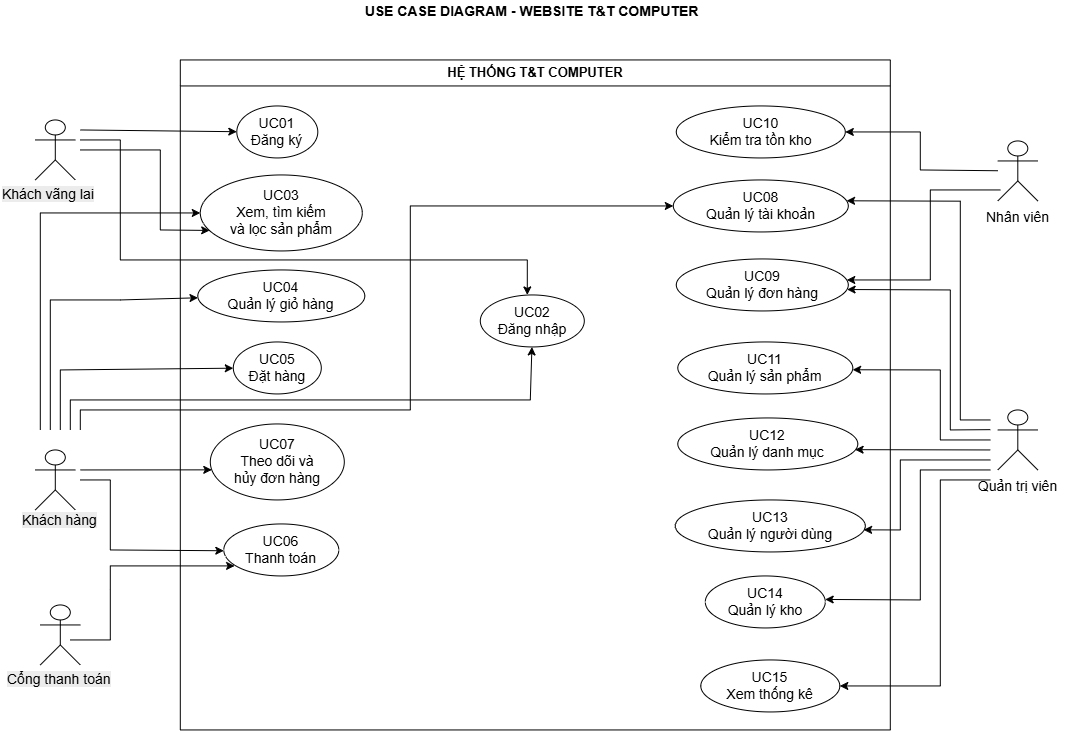
\includegraphics[width=\textwidth]{UseCase.png}}{\fbox{\parbox{0.9\textwidth}{\centering Không tìm thấy tệp UMLtongquat.png}}}

 \caption{Biểu đồ Use Case tổng quát}

 \label{fig:usecase-tongquat}

\end{figure}
\newpage
\section{Biểu đồ Class tổng quát}

Biểu đồ Class tổng quát của hệ thống website T\&T COMPUTER

được sử dụng để mô tả các lớp, thuộc tính, phương thức và mối quan hệ

giữa các lớp trong hệ thống.

\begin{figure}[H]

    \centering

    \IfFileExists{class.png}{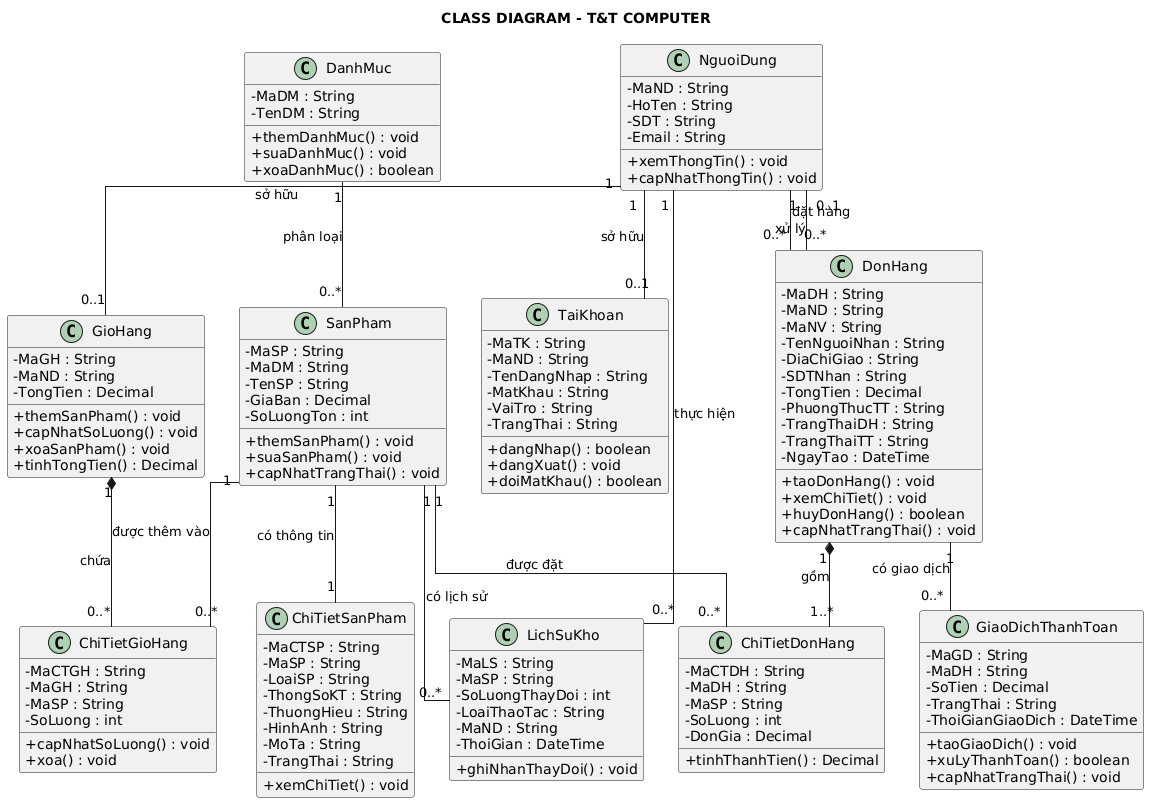
\includegraphics[width=\textwidth]{class.png}}{\fbox{\parbox{0.9\textwidth}{\centering Không tìm thấy tệp class.png}}}

    \caption{Biểu đồ Class tổng quát}

    \label{fig:class-tongquat}

\end{figure}
\newpage
\section{Biểu đồ Database tổng quát}

Biểu đồ Database tổng quát của hệ thống website T\&T COMPUTER

được sử dụng để mô tả các bảng dữ liệu, thuộc tính và mối quan hệ

giữa các bảng trong cơ sở dữ liệu của hệ thống.

\begin{figure}[H]

    \centering

    \IfFileExists{database.png}{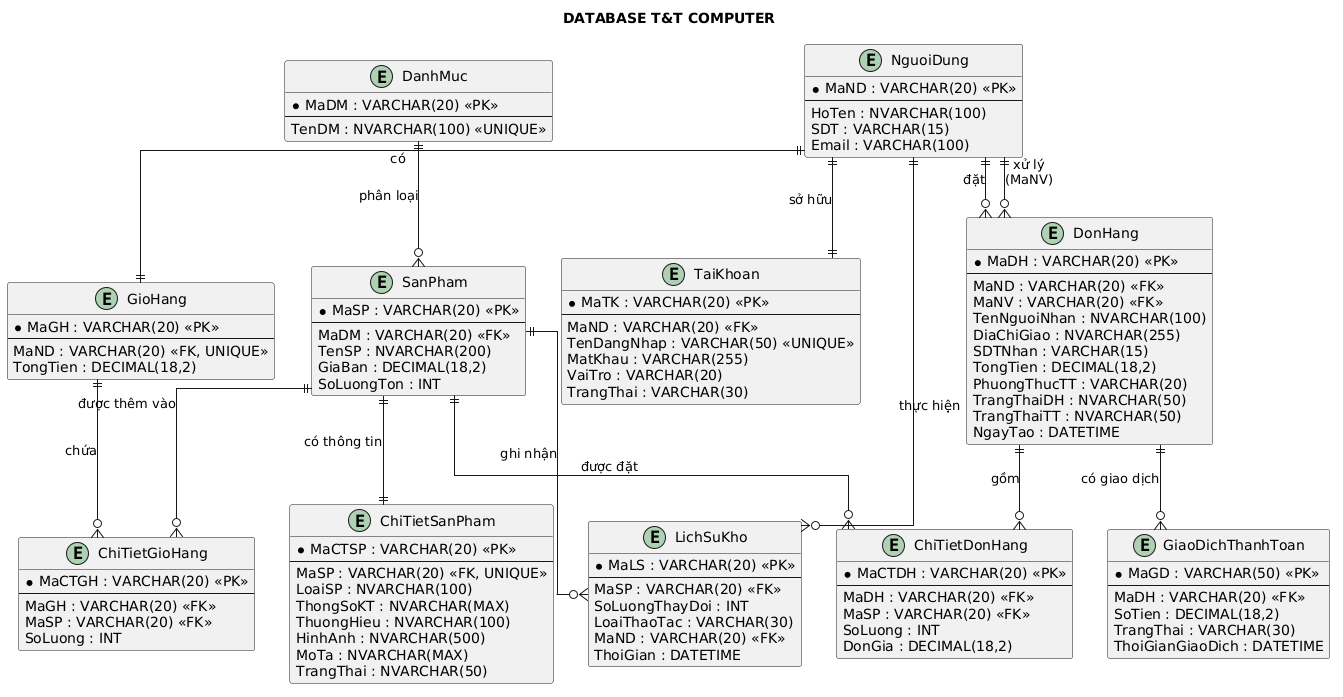
\includegraphics[width=\textwidth]{database.png}}{\fbox{\parbox{0.9\textwidth}{\centering Không tìm thấy tệp database.png}}}

    \caption{Biểu đồ Database tổng quát}

    \label{fig:database-tongquat}

\end{figure}

\end{document}
